% Compile with pdfLaTeX.
% Landscape version corresponding to the revised portrait template.
% Font matching is intentionally relaxed for this version.

\documentclass[a4paper,landscape]{article}

% Scroll down to line 74

% Minimal external packages:
\usepackage[a4paper,landscape,left=18mm,right=18mm,top=18mm,bottom=18mm]{geometry}
\usepackage{graphicx}
\usepackage{xcolor}
\usepackage{lipsum}
\usepackage{array}
\usepackage[T1]{fontenc}
\usepackage[sfdefault]{roboto}
\usepackage[
    colorlinks=true,
    urlcolor=blue,
    linkcolor=black,
    citecolor=blue
]{hyperref}

\pagestyle{empty}
\setlength{\parindent}{0pt}
\setlength{\parskip}{0pt}
\setlength{\tabcolsep}{0pt}
\definecolor{topicblue}{HTML}{2F5597}

% Lengths - specifications for template fonts, appearance
\newlength{\HeaderSize}
\setlength{\HeaderSize}{24pt}
\newlength{\HeaderSizeBaseline}
\setlength{\HeaderSizeBaseline}{28.8pt}

\newlength{\SectionSize}
\setlength{\SectionSize}{16pt}
\newlength{\SectionSizeBaseline}
\setlength{\SectionSizeBaseline}{1.2\SectionSize}

\newlength{\TextSize}
\setlength{\TextSize}{14pt}
\newlength{\TextSizeBaseline}
\setlength{\TextSizeBaseline}{1.3\TextSize}

\newlength{\CaptionSize}
\setlength{\CaptionSize}{12pt}
\newlength{\CaptionSizeBaseline}
\setlength{\CaptionSizeBaseline}{1.2\CaptionSize}

\newlength{\RefSize}
\setlength{\RefSize}{12pt}
\newlength{\RefSizeBaseline}
\setlength{\RefSizeBaseline}{1.4\RefSize}

\newlength{\vskipHeader}
\setlength{\vskipHeader}{8.0mm}
\newlength{\vskipSection}
\setlength{\vskipSection}{4.0mm}
\newlength{\vskipText}
\setlength{\vskipText}{2.0mm}
\newlength{\vskipImage}
\setlength{\vskipImage}{16.0mm}

% Landscape geometry.
% The left panel is square; the right panel uses the remaining width.
\newlength{\LeftPanel}
\setlength{\LeftPanel}{164mm}
\newlength{\PanelGap}
\setlength{\PanelGap}{18mm}
\newlength{\RightPanel}
\setlength{\RightPanel}{79mm}

% Do not change anything above this line!

\begin{document}
\noindent
\begin{tabular}{@{}p{\LeftPanel}@{\hspace{\PanelGap}}p{\RightPanel}@{}}

% ======================= LEFT SQUARE =======================
\parbox[t][\LeftPanel][t]{\LeftPanel}{%

% High page header
\begin{center}
  {\fontsize{\HeaderSize}{\HeaderSizeBaseline}\selectfont\color{topicblue}%
  %
  % Agnese will modify this; For now write your name and number your projects with 1 and 2
   Project Topic:\hspace{9mm} (Xinwen 2)} 
\end{center}

\vspace{\vskipHeader}

% Main title
{\fontsize{\SectionSize}{\SectionSizeBaseline}\selectfont\bfseries 
%
% Title
Network Heterogeneity and Epidemic Spreading
\par}
\vspace{\vskipSection}

% Abstract / project description --> adjust accordingly
{\fontsize{\TextSize}{\TextSizeBaseline}\selectfont
%
% Intro+Motivation
The spread of infectious diseases depends strongly on the pattern of contacts between individuals. Classical epidemic models often assume a well-mixed population, but real populations are heterogeneous: some individuals have many contacts, others have few, and contacts are often clustered within families, workplaces, or social groups. Networks represent this structure naturally, with individuals as nodes and potentially infectious contacts as edges (Fig. 1). Network structure can strongly affect epidemic dynamics [1]: highly connected individuals may promote transmission, while clustering may keep infections within local groups. Thus, populations with the same average number of contacts can still experience very different outbreaks if their degree distributions or clustering differ.
\par

\vspace{\vskipText}
% In this project
In this project, you will investigate how network topology affects the spread of an SIR-type infectious disease. You will generate networks with different degree distributions and clustering levels and simulate stochastic disease transmission on them. 
\par
}

\vfill
\vspace{\vskipSection}
% References are entered manually. No .bib file / BibTeX / biblatex.
{\fontsize{\SectionSize}{\SectionSizeBaseline}\selectfont\bfseries References:\par}
\vspace{\vskipSection}

{\fontsize{\RefSize}{\RefSizeBaseline}\selectfont
% 
% Reference 1
[1] Pastor-Satorras, R., et al.
\textit{Epidemic processes in complex networks}, Rev. Mod. Phys. \textbf{87(3)}, 925–979 (2015).\\
\href{https://doi.org/10.1103/RevModPhys.87.925}{https://doi.org/10.1103/RevModPhys.87.925} 
\par
% 

% Add Reference 2 (if needed)
\par
% 
% Add a Reference 3 (if needed)
\par
}
\vspace{\vskipText}
}% end left square

&

% ======================= RIGHT COLUMN =======================
\parbox[t][\LeftPanel][c]{\RightPanel}{%
\centering
%
% Representative image + caption. 
\begin{tabular}{@{}c@{}}
%
% Image
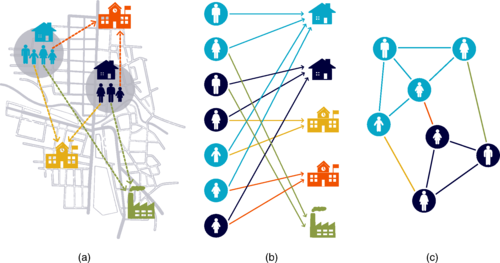
\includegraphics[width=\RightPanel]{medium.png}\\[\vskipSection] % name of the image 
\parbox{\RightPanel}{%
\fontsize{\CaptionSize}{\CaptionSizeBaseline}\selectfont
\textbf{Fig.1}\quad 
% 
% Title of the image (bold)
\textbf{Schematic illustration of the construction of a synthetic population and the resulting contact network [1]} 
% 
% Body of the image caption.
(a) A synthetic population and its movements are built from census and demographic data. (b) These data are used to create a bipartite network linking individuals to locations, with links optionally weighted by time spent there. (c) Projecting this network produces a contact network for contagion, with transmission rates and link weights varying by location and interaction type.
%
% Credits.

}
\end{tabular}
}% end right column

\end{tabular}
\end{document}
